\chapter{Metodologias}
\label{chap:metodologia}
Nesta seção serão apresentadas as metodologias usadas para o desenvolvimento desse trabalho. As etapas a serem seguidas estão representadas no fluxograma da Figura \ref{fig:etapas}.

\begin{figure}[ht]
  \centering
  \captionsetup{width=16cm}
  \caption{Fluxograma das etapas}
  \label{fig:etapas}
  \tcbox[left=0cm, right=0cm, top=0cm, bottom=0cm,center]{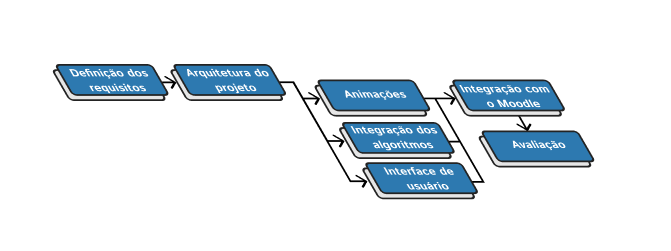
\includegraphics[width=15.6cm]{figuras/fluxograma.png}}
  \Fonte{fornecida pelo próprio autor}
\end{figure}
%\FloatBarrier

\section{Definir os requisitos}
A partir da revisão bibliográfica foram definidos alguns requisitos básicos que deveriam estar presentes na ferramenta. Como requisito não funcional foi definido oferecer suporte multi-plataforma, para \textit{mobile}, \textit{desktop} e \textit{web}. Como requisitos funcionais foram definidos os seguintes:
\begin{itemize}[label={$\sbullet$}]
    \item Permitir que os usuários digitem a gramática a ser analisada.
    \item Permitir que os usuários visualizem o estado das estruturas dos algoritmos.
    \item Permitir que os usuários avancem, retornem e reiniciem os passos da execução dos algoritmos.  
    \item Permitir que os usuários selecionem o algoritmo a ser visualizado.
\end{itemize} 
 
Apesar das ferramentas compartilharem as mesmas funcionalidades básicas já definidas inicialmente, outras têm características interessantes que podem ser reaproveitadas, partir delas foram definidos os seguintes requisitos:
\begin{itemize}[label={$\sbullet$}]
    \item Permitir que os usuários digitem uma \textit{string} a ser analisada.
    \item Permitir que os usuários visualizem a análise de uma \textit{string}.
    \item Permitir que os usuários visualizem a árvore sintática de uma \textit{string}. 
    \item Permitir que os usuários copiem em formato de texto os resultados da análise de uma \textit{string}.
    \item Permitir que os usuários copiem implementações dos algoritmos. 
\end{itemize}

Com esses requisitos tem-se a base para o desenvolvimento da ferramenta.

\section{Definir a arquitetura do projeto}
O projeto será construído usando o \textit{framework Svelte}, sem \gls{ssr}, para que seja possível o funcionamento \textit{offline} da ferramenta, já que a ferramenta não teria acesso ao servidor não seria possível usá-lo para renderizar elementos. \textit{Svelte} compila a base de código e cria uma coleção de arquivos estáticos que constituem a página \textit{web} e a base para o suporte multi-plataforma da aplicação.
\begin{figure}[ht]
  \centering
  \captionsetup{width=16cm}
  \caption{Arquitetura da aplicação em nuvem}
  \label{fig:arqremo}
  \tcbox[left=0cm, right=0cm, top=0cm, bottom=0cm,center]{
    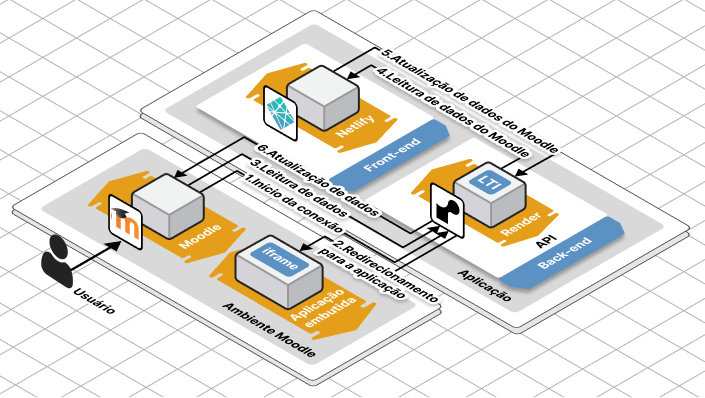
\includegraphics[width=15.6cm]{figuras/remote.png}}
  \Fonte{fornecida pelo próprio autor}
\end{figure}

O \textit{framework Capacitor} consome essa coleção de arquivos e cria um projeto para plataforma \textit{Android} que é usado para criar a versão \textit{mobile} da ferramenta usando o \textit{Android Studio}. O \textit{framework Tauri} constrói instaladores para \textit{desktop} diretamente da coleção de arquivos estáticos. A plataforma alvo dos instaladores é a plataforma na qual eles são construídos, já que o \textit{framework} não tem suporte para construção \textit{cross-platform} é necessária a utilização de máquinas virtuais para construir instaladores para diferentes plataformas \textit{desktop}.

Para a versão \textit{online} da aplicação, os serviços de computação em nuvem das empresas \textit{Netlify} e \textit{Render} serão usados para hospedar respectivamente o \textit{front-end} e \textit{back-end} da aplicação. \textit{Netlify} e \textit{Render} foram escolhidas para hospedagem da aplicação pelo oferecimento gratuito dos serviços para aplicações pequenas como a proposta nesse trabalho.

A aplicação pode ser acessada através do \textit{Moodle} usando como comunicação entre os dois a \gls{api} da aplicação. O diagrama na Figura \ref{fig:arqremo} mostra o esquema da arquitetura da aplicação hospedada em nuvem com integração ao \textit{Moodle}. A versão hospedada localmente da aplicação segue a mesma arquitetura com exceção da utilização de serviços de computação em nuvem.


%\FloatBarrier

\section{Implementar a interface de usuário}
Para que o usuário selecione um algoritmo para visualizar a ferramenta terá opções no topo da tela que alternam entre abas. Dentre essas abas estarão inclusas uma para a entrada de gramáticas e uma aba para visualização de cada algoritmo disponível. Para que o usuário possa dar uma gramática de entrada será criado um campo de texto como mostra Figura \ref{fig:mgrammar}.

\begin{figure}[ht]
    \centering
    \captionsetup{width=16cm}
    \caption{Aba de entrada da gramática}
    \label{fig:mgrammar}
    \tcbox[left=0cm, right=0cm, top=0cm, bottom=0cm,center]{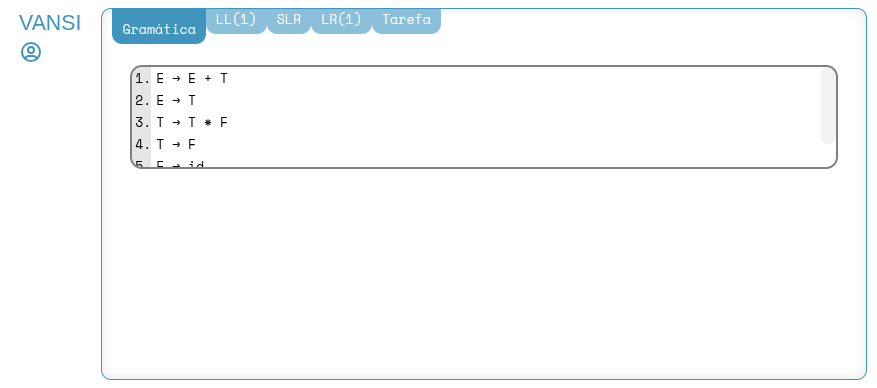
\includegraphics[width=15.6cm]{figuras/mgrammar.png}}
    \Fonte{fornecida pelo próprio autor}
\end{figure}
%\FloatBarrier

Para a visualização dos algoritmos a ferramenta terá uma composição de elementos como mostra a Figura \ref{fig:mfirst}, esses elementos são modificados de acordo com a execução do algoritmo selecionado. Os passos da execução do algoritmo podem ser controlados pelo conjunto de controles acima dos elementos do algoritmo como mostra a Figura \ref{fig:mfirst}.

\begin{figure}[ht]
    \centering
    \captionsetup{width=16cm}
    \caption{Aba de visualização dos algoritmos}
    \label{fig:mfirst}
    \tcbox[left=0cm, right=0cm, top=0cm, bottom=0cm,center]{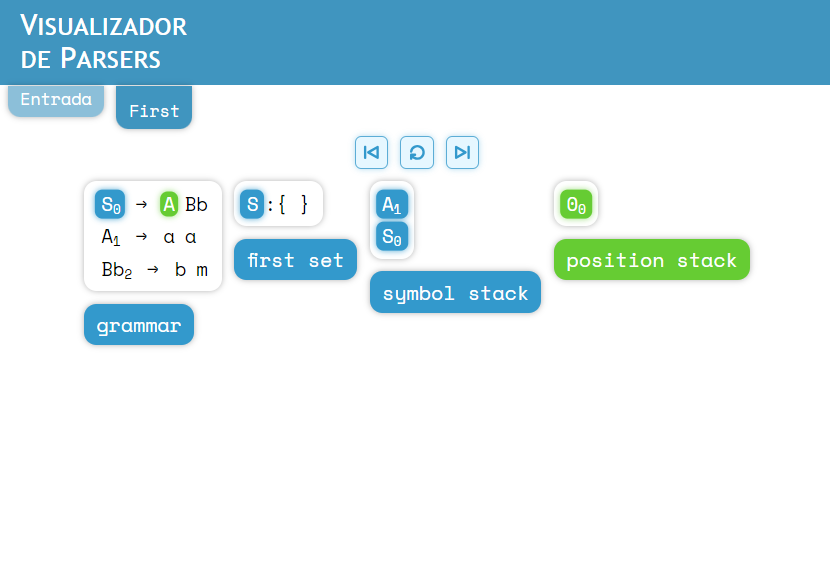
\includegraphics[width=15.6cm]{figuras/mfirst.png}}
    \Fonte{fornecida pelo próprio autor}
\end{figure}
%\FloatBarrier

Nas abas de visualização de algoritmos serão inclusos um campo de texto no qual o usuário poderá inserir uma \textit{string} de entrada para ser analisada pelo algoritmo, um campo de texto para copiar os resultados dos algoritmos em forma de texto e um campo de texto para copiar a implementação do algoritmo.

\section{Integrar os algoritmos à ferramenta}
Para todas as estruturas de dados usadas nos algoritmos serão criadas representações visuais, dessa forma todos os passos do funcionamento poderão ser representados como estados dessas estruturas. Calculando antecipadamente os estados dessas estruturas em cada passo dos algoritmos podemos fazer um controle de fluxo entre os passos dos algoritmos.

\section{Implementar as animações dos algoritmos}
As mudanças de estados que ocorrem nos algoritmos podem ser melhor compreendidas se poderem ser visualizadas como transições ao invés de mostrar as mudanças saltando do estado inicial para o estado final. Usar animações torna a visualização das mudanças muito mais dinâmica. Um exemplo de animação é a animação do estado da estrutura de pilha que é usada em alguns algoritmos. Quando um item é adicionado ou removido da pilha, o elemento visual que representa esse item terá sua posição interpolada do ponto inicial ao ponto final.

\section{Integrar a ferramenta com o \textit{Moodle}}
A plataforma \gls{lms} \textit{Moodle} implementa o padrão \gls{lti} o que permite a utilização da ferramenta criada nesse trabalho diretamente no \textit{Moodle} sem necessidade de \textit{login} externo. Para que a ferramenta possa utilizar o padrão \gls{lti} com o \textit{Moodle} será implementado no \textit{back-end} da aplicação uma \gls{api} que manuseia as requisições relacionada ao \gls{lti}. 

Os \textit{endpoints} da \gls{api} foram definidos de acordo com o Quadro \ref{qua:endpoints}.

\setlength{\abovecaptionskip}{10pt plus 0pt minus 0pt}
\setlength{\belowcaptionskip}{5pt plus 0pt minus 0pt}
\begin{table}[h]
\centering\setlength{\extrarowheight}{2pt}
\captionsetup{width={\textwidth}}
\captionof{quadro}{Endpoints}\label{qua:endpoints}
\resizebox{\textwidth}{!}{
\begin{NiceTabular}{m[c]{3cm}m[c]{3cm}m[c]{10cm}}[corners,hvlines]
\CodeBefore
  \rowcolor{gray!15}{1-1}
\Body
\textbf{Endpoint} & \textbf{Método} & \textbf{Finalidade}  \\
\selectlanguage{brazil}$\backslash$\selectlanguage{brazil}& GET & redirecionar para página\\
\selectlanguage{brazil}$\backslash$\selectlanguage{brazil}login & POST & inicia uma conexão com a plataforma\\
\selectlanguage{brazil}$\backslash$\selectlanguage{brazil}register & POST & registrar uma nova plataforma\\
\end{NiceTabular}}
{\Fonte{fornecido pelo autor}}
\end{table}

Com a \gls{api} pronta pode ser feita a conexão entre a ferramenta e a \gls{lms}. Utilizando o serviço \gls{lti} de \textit{Dynamic Registration} é possível fazer o cadastro da ferramenta no \textit{Moodle} utilizando um \textit{link} para o \textit{endpoint} de registro dinâmico da \gls{api}.

\section{Avaliar a ferramenta}
Será realizado um teste prático com um grupo de estudantes, onde os eles serão solicitados a realizar tarefas específicas utilizando a ferramenta. Serão coletados dados quantitativos, como tempo de execução das tarefas e taxa de acerto, bem como dados qualitativos por meio de questionários e entrevistas para avaliar a percepção dos estudantes sobre a eficácia da ferramenta. Além disso, a comparação dos resultados obtidos com um grupo de controle que não utiliza a ferramenta ajudará a avaliar o impacto da visualização na compreensão e desempenho dos alunos. Essa abordagem abrangente de avaliação garantirá uma análise completa da eficácia e utilidade da ferramenta desenvolvida nesse trabalho.

O desenvolvimento desse trabalho seguirá o cronograma mostrado no Quadro \ref{qua:cronograma}.
\setlength{\abovecaptionskip}{10pt plus 0pt minus 0pt}
\setlength{\belowcaptionskip}{5pt plus 0pt minus 0pt}
\begin{table}[h]
\centering\setlength{\extrarowheight}{2pt}
\captionsetup{width={\textwidth}}
\captionof{quadro}{Cronograma}\label{qua:cronograma}
\resizebox{\textwidth}{!}{\begin{NiceTabular}{l*{6}{c}}[corners,hvlines]
\CodeBefore
  \rowcolor{gray!15}{1-3}
\Body
\Block{3-1}{Atividades}  & \Block{1-6}{Período}  \\
&\Block{1-3}{2024}& &&\Block{1-3}{2025} \\
&Outubro&Novembro&Dezembro&Janeiro&Fevereiro&Março\\

Definir dos requisitos                &x& & & & & \\
Definir arquitetura do projeto        &x& & & & & \\
Implementar da interface de usuário   & &x&x& & & \\
Integrar os algoritmos                & & &x&x&x& \\
Implementar as animações              & & &x&x&x& \\
Integrar ao Moodle                    & & & &x&x& \\
Avaliar a ferramenta                  & & & & &x& \\
Escrita do TCC II                     &x&x&x&x&x&x\\
Defesa do TCC II                      & & & & & &x\\
\end{NiceTabular}}
{\Fonte{fornecido pelo autor}}
\end{table}
